\chapter{Detailed design}

\section{Actor model}

In each module we can detect few different components that may interact in a very complex way. Moreover, each component may own more than one control flow. This could lead to a growth in design complexity and to potential concurrency issues to be solved.
\\
In order to cut those aspects down, components are organized using an actor model. This way, components can be seen as self-contained services that communicate using message passing.
\\
The only drawback is the exposure of the actor model to users that may be forced to think in term of a non trivial programming paradigm. In order to prevent that, library logic and structure is hidden behind an interface layer. This can be achieved just by using a simple facade pattern that permits to mask actor model and message passing by using the solely asynchronous programming, simpler to users the may not know the actor model and more general for users that wouldn't structure their programs using actors.

\section{Room}

Room is one of the main concept of the library, both on server and client perspective; the figure \ref{fig:room_class_diagram} shows its design.
\\
\texttt{Room} is the primary interface that defines a room. A room has a unique identifier and a set of properties. The identifier is an UUID string that can be used by clients to reference a specific room. On the other hand, properties (described in section \ref{room_properties_section}) can be queried to retrieve some useful information exposed by the room.
Both \texttt{ClientRoom} and \texttt{ServerRoom} extend \texttt{BasicRoom}, the one that provides common methods to access properties.
 \\
\texttt{SharedRoom} is the serializable object that is passed through the network to share room information between clients and server.
\\
The following sections provide a more detailed description of client and server specializations of the room concept, focusing on \texttt{ClientRoom} and \texttt{ServerRoom} classes.



\begin{figure}
	\centering
	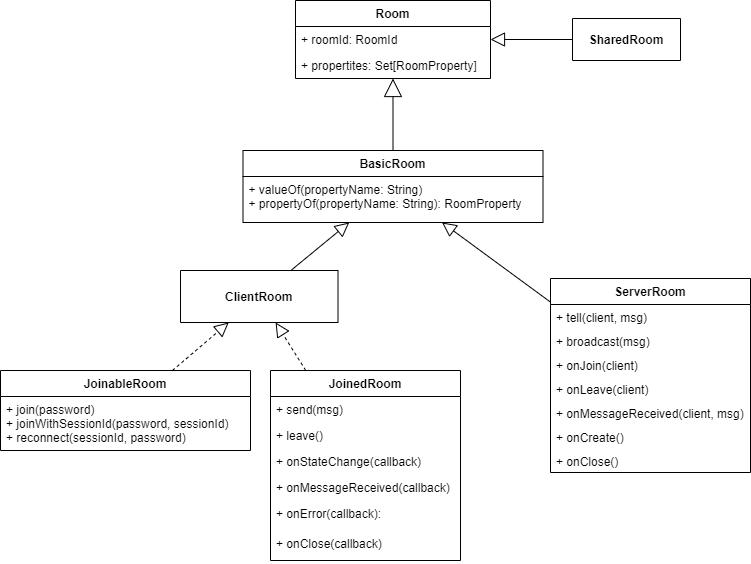
\includegraphics[scale=0.5]{images/4-design/room-class.png}
	\caption{Room class diagram}
	\label{fig:room_class_diagram}
\end{figure}

\subsection{ServerRoom}
\begin{figure}
	\centering
	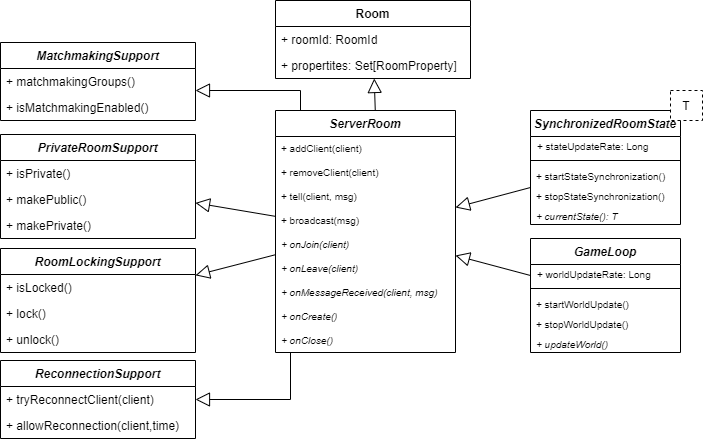
\includegraphics[scale=0.5]{images/4-design/server-room.png}
	\caption{Server room class diagram}
	\label{fig:server_room_class_diagram}
\end{figure}

\texttt{ServerRoom} is a trait that encapsulates the concept of room used server-side; as we see in figure \ref{fig:server_room_class_diagram}, it extends the \texttt{Room} trait by adding methods to manage clients (add, remove, tell and broadcast) and by defining abstract handlers for room events. These handlers are the ones that the developer must implement to define his own type of room.
\\
Few extensions are provided to enhance its functionalities, in particular:

\begin{itemize}
    \item \texttt{MatchmakingSupport}: it gives the developer access to the matchmaking groups created by the matchmaking service associated with this room.
	\item \texttt{PrivateRoomSupport}: it manages private rooms by allowing the possibility to set a password to the room in order to prevent undesired accesses.
	\item \texttt{RoomLockingSupport}: it enables lock and unlock functionalities to the room.
	\item \texttt{ReconnectionSupport}: it allows clients reconnection to the room.
	\item \texttt{SynchronizedRoomState}: it permits to synchronize the public state of the room between clients using a period of \texttt{stateUpdateRate}.
	\item \texttt{GameLoop}: it permits to update the room state using a period of \texttt{stateUpdateRate}.
\end{itemize}

Differently from the others, \texttt{SynchronizedRoomState} and \texttt{GameLoop} are optionals and can be included by the developer at will.

The first one is a trait generic in the type of the state that needs to be synchronized to clients; all methods are implemented, except for \texttt{currentState} that must be defined by the user. This method should return the new world to be synchronized between the clients.

The latter is also a trait and requires to define \texttt{updateWorld}, a method that is assigned to update the room using a given logic.

\subsection{ClientRoom}

\texttt{ClientRoom} is the client-side representation of the room.
This concept has been then specialized in two further concepts: ``Joinable'' and ``Joined''.
This separation was made to provide the developer a consistent access to room functionalities. Indeed, by using this structure, it is not possible to execute unauthorized operations on rooms. For example, leaving a room that wasn't joined yet or joining a room that is already joined.

\bigskip
\texttt{JoinableRoom} extends a basic \texttt{ClientRoom} and adds join and reconnect accessing protocols.


\bigskip
\texttt{JoinedRoom} extends the \texttt{ClientRoom} trait too and enables the definition of callbacks on room events: message received, state changed, room closing or communication error.
Furthermore, it also exposes methods to send messages and leave the room.
\\
A client is provided with a \textit{sessionId} that identifies the joining of the client to the room.
This can be used, for example, in the reconnection process in order to recognize the client on the server.


\subsection{Properties and Filters}  \label{room_properties_section}
UML class diagram in figure \ref{fig:property-class} shows the detailed architecture of room properties and filters.

\bigskip
\textit{Basic room properties}
\\
Each property (\texttt{BasicRoomProperty}) owns a name and a value.
\\
Values, since they can be of four types (server requirements 2.2.2), are modeled as classes that extend a common trait \texttt{RoomPropertyValue}. This trait wraps a ``real'' value of type \texttt{Int}, \texttt{Double}, \texttt{Boolean} or \texttt{String}.
\\
Each property value exposes two main features: the real value wrapped by the class and a method that compares such value to another one of the same type (e.g. compare the \texttt{Int} value wrapped by the class to another given \texttt{Int}); this is useful since different type of values may define different comparing logics.
Moreover, there is also a static factory that permits to create a property value from a given first class value (if possible).

\bigskip
\textit{Filters}
\\
By looking to client requirement 1.6.1, there are four available filter strategies. Similarly to property values, they are hidden behind a common trait \texttt{FilterStrategy}. Such trait defines a name for the strategy and an evaluation predicate that permits to apply the strategy to two values. The evaluation result expresses if the filtering defined by the strategy is satisfied.

\bigskip
Since library usability is a core aspect, a simple DSL language is created in order to easily manage filters.
\\
\texttt{BasicRoomProperty} functionalities are extended to include filters by using mixins. This way, filter strategies can be directly called by the property itself.
\\
A \texttt{FilterOption} is something that contains the name of the property to be filtered, the strategy to be uses and a value the property should be compared to. It exposes an utility method to concatenate two \texttt{FilterOption} too.
\\
A \texttt{FilterOptions} is a wrapper around a set of \texttt{FilterOption}; this is useful when talking about DSL since it permits to define static factories (\texttt{empty}, \texttt{just}) and utility methods such as concatenation (\texttt{and}) and union (\texttt{++}).

\bigskip
\textit{Design notes / implementation directives}
\\
\begin{itemize}
\item Before on choosing this design, few different options have been analyzed, and this has been decided to be the most feasible one. The only lack that can be detected is on the value getter of \texttt{RoomPropertyValue}. Indeed, it is absent in the class instance itself, and it is only available through the static method \texttt{valueOf}.
\item Notice that, in order to encourage library usability, the value wrapper can be made be transparent to final users thanks to implicit conversions that can be defined in Scala.
\end{itemize}

\begin{figure}[h]
	\hspace*{-0.1in}
	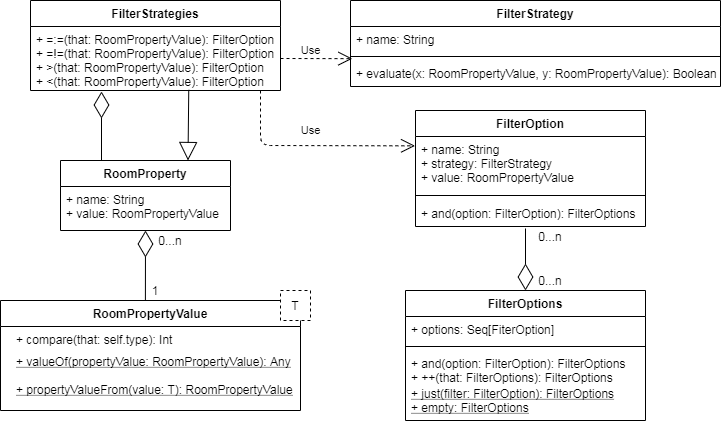
\includegraphics[scale=0.55]{images/4-design/property_and_filters-class.png}
	\caption{Properties and filters class diagram.}
	\label{fig:property-class}
\end{figure}


\section{Server}
Class diagram in figure \ref{fig:server_class_diagram} describes in detail the server architecture by describing its main functionalities and by showing its components interactions.
\begin{figure}[h]
	\hspace*{-1.1in}
	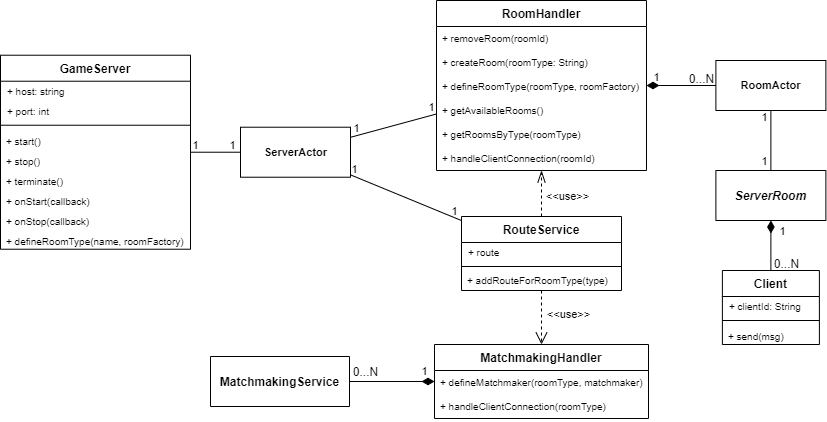
\includegraphics[scale=0.55]{images/4-design/server_class.png}
	\caption{Server class diagram}
	\label{fig:server_class_diagram}
\end{figure}

\textit{Game server and routing service}
\\
The \texttt{GameServer} class is the facade interface that is exposed to the developer. It internally creates a \texttt{ServerActor} that is the entity acting as the real server listening for clients requests. This actor creates a \texttt{RouteService} object that is used to know which routes to use and how to handle requests; it also allows to dynamically define new room types that will be used by the server.

The \texttt{ServerActor} also uses a \texttt{RoomHandlingService} actor to create and define rooms from the server itself. The same actor is used by the \texttt{RouteService}.

\bigskip
\textit{Rooms and room handling service}
\\
As we described for the server architecture in section \ref{sec:server_arch}, the purpose of the \texttt{RoomHandlingService} is to manage the active rooms in the application. Specifically, it doesn't directly create rooms; instead, it creates \texttt{RoomActor}(s), namely actors used as ``wrappers'' for \texttt{ServerRoom}(s) to avoid concurrency issues and to semplify the overall system design. This is required since more than one client can interact with a single room at the same time and so, in order to avoid race conditions, clients communicate with \texttt{RoomActor}(s) that process messages sequentially. Each actor is in charge of notifying clients' actions to the room it is associated with.

\bigskip
\textit{Client}
\\
Each \texttt{ServerRoom} is linked to an actor and keeps track of connected clients (\texttt{Client} class server-side). Clients are uniquely identified by their Id and expose a \texttt{send} method that allows to send messages to them. It is important to notice that each room has its own view of clients: the same client connected to different rooms will have a different Id in each of them.

\bigskip
\textit{Matchmaking}
\\
Each matchmaking service has an internal actor assigned to handle all incoming requests. This actor needs to know which \texttt{Client}(s) are waiting for the match start.
Since clients may ask for matchmaking, the \texttt{RouteService} uses a \texttt{MatchmakingHandler} to redirect those requests to the right \texttt{MatchmakingService} actor.
Moreover, when defining a new room type with enabled matchmaking, the server will demand the \texttt{RouteService} to add the right route and to spawn the associated \texttt{MatchmakingService}.


\section{Client}

Class diagram in figure \ref{fig:client_class_diagram} describes the detailed client architecture.

\bigskip
\textit{Core client}
\\
The \texttt{Client} class is the main access point to its api. It's a facade that exposes client's primary functionalities while hiding the underlying actor model.
\\
The main logic is internally handled by the \texttt{CoreClient} actor. It exploits an \texttt{HttpService} actor to make http requests to the game server when getting or creating rooms.
\\
Moreover, it keeps track of currently joined rooms. The list, once created, is kept updated by interacting with the \texttt{ClientRoomActor}'s associated with each room.

\bigskip
\textit{Client room}
\\
The \texttt{ClientRoomActor} is an actor that handles the socket connection with the server side room. 
It's spawned when joining a room, and it's killed when the room is left or closed. It notifies the \texttt{CoreClient} when the associated room is left, joined or closed so that the list of joined rooms can be updated.
\\
In the end, the callbacks specified by the user, i.e. the ones that define the client side room reactive behavior, are handled by this actor internally.

\bigskip
\textit{Matchmaking}
\\
The \texttt{ClientMatchmaker} can be used to access the matchmaking functionality. It exposes methods to join or leave matchmaking queues for given room types. It keeps track of active matchmaking connections so that it is always possible to leave queues without waiting the matchmaking process to be completed.
\\
A \texttt{MatchmakingActor} is spawned when a new matchmaking request is performed.
This actor opens a websocket connection with the server side matchmaker and notifies the client after the the joinin operation on the room created by the matchmaking service. This actor is killed when the matchmaking process completes or the relative matchmaking queue is left.

\begin{figure}
	\hspace*{-1 in}
	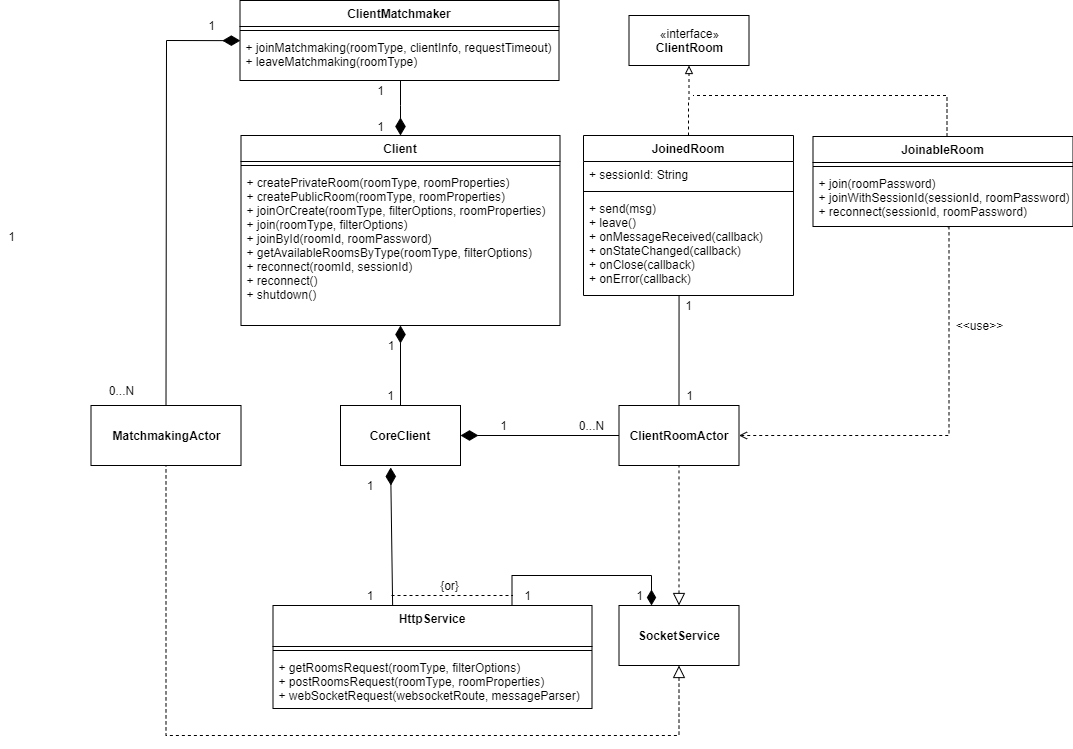
\includegraphics[scale=0.55]{images/4-design/client_class.png}
	\caption{Client class diagram}
	\label{fig:client_class_diagram}
\end{figure}

\section{Communication}\label{sec:communication_design}


\subsection{Json Serialization}
For Request-Response interaction (described in section 3.4), Json format has been used for client requests and server responses both. \texttt{RoomJsonSupport} class provides json-formatted serialization capabilities for all entities that are exchanged at this stage of client-server interaction, in particular:
\begin{itemize}
	\item \texttt{SharedRoom} objects and related (e.g. roomId).
	\item Room properties and related/derivatives (e.g. set of properties, property value).
	\item Room filters and related/derivates (e.g. filter strategies, \texttt{FilterOptions}).
\end{itemize}

\subsection{Websockets}
\begin{figure}[h]
	\hspace*{-0.5in}
	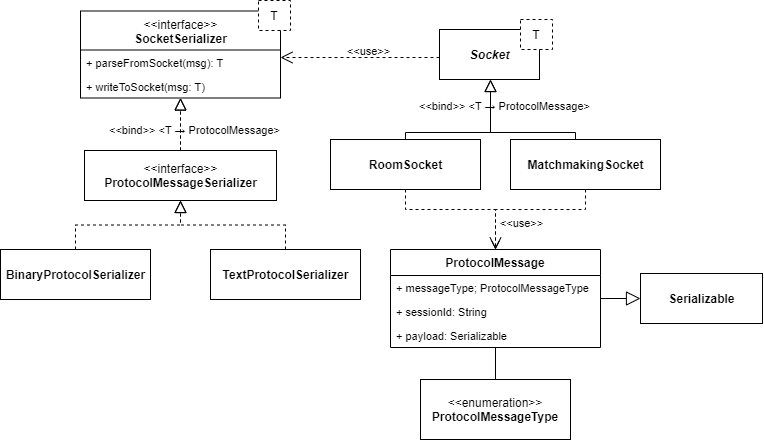
\includegraphics[scale=0.6]{images/4-design/communication_protocol.png}
	\caption{Websocket class diagram}
	\label{fig:websocket_communication_design}
\end{figure}
Regarding websockets, a class diagram describing the main classes is shown in figure \ref{fig:websocket_communication_design}.
The \texttt{Socket} abstract class provides the main functionalities for a socket communication and allows to define the configuration for the connection (heartbeat rate, idle timeout). It is generic in T where T represents the type of messages sent through that socket . Two concrete implementations are provided for this class:
\begin{itemize}
	\item \texttt{RoomSocket}: used for the communication between client and rooms.
	\item \texttt{MatchmakingSocket}: used for the communication between client and matchmaking services.
\end{itemize}
They are \texttt{Socket} both where the generic type T is a \texttt{ProtocolMessage}. Indeed, this is the class that defines the communication protocol between client and server. It uses a structure made up of three fields to describe a message sent through a socket:
\begin{itemize}
	\item \textit{MessageType} \\
	Used to identify the type of message that the client or the server want to send. The list of the possible message types is defined in the \texttt{ProtocolMessageType} enumeration.
	\item \textit{SessionId} \\
	Used to identify the client that is sending the message through the socket. When a websocket connection is established between client and server, a unique Id is generated; the client must always use the same sessionId to send messages through that socket.
	\item \textit{Payload} \\
	An optional payload that can be carried with the massage. This is, for example, the field used to store messages when a client sends a message to the server through the usage of \texttt{sendMessage} method on the client room. It must be \texttt{Serializable} since it will eventually be serialized to be sent to the server.
\end{itemize}

In order for a \texttt{Socket} object to send and receive data, it must be able to serialize and deserialize messages that pass through it. It uses for this purpose a \texttt{SocketSerializer} that has two methods: \texttt{parsefromSocket} and \texttt{writeToSocket}. This class is generic in T that is the type of messages that needs to be read and written.

Since \texttt{RoomSocket} and \texttt{MatchmakingSocket} need to handle \texttt{ProtocolMessage}(s), a \texttt{ProtocolMessageSerializer} interface specifically defines a serializer for protocol messages. Two types of serializers are implemented: \texttt{BinaryProtoclSerializer} and \texttt{TextProtocolSerializer}. The first one serializes protocol messages as binary data, the latter, instead, as text messages.
 
Two different implementations are present because Json format may be also used for socket communication by exploting the \texttt{TextProtocolSerializer}. However, the binary representation improves performance and usability both (a developer just needs to extend \texttt{java.io.Serializable} vs. create a Json parser using \texttt{spray.sjon.RootJsonFormat}). Hence, at the moment, the binary representation is the used one, and the Json format is kept just because of its usefulness in testing purposes.

\bigskip
Sequence diagram in figure \ref{fig:create_room_seq} shows an example of full interaction between client and server. Specifically, it represents a client request about the creation of a new room.

\begin{figure}
	\hspace*{-1in}
	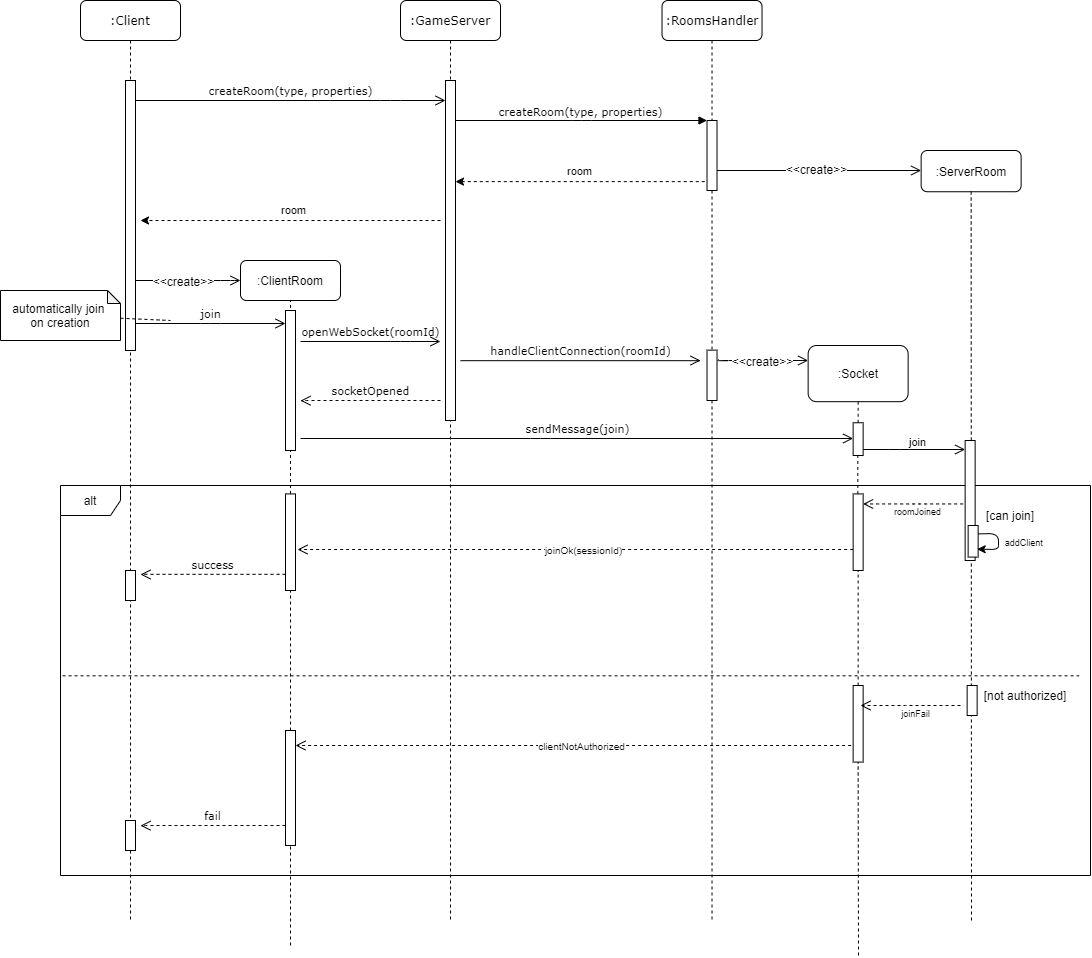
\includegraphics[scale=0.5]{images/4-design/create_room_seq.png}
	\caption{Example of a client-server interaction upon a 'create room' request}
	\label{fig:create_room_seq}
\end{figure}